\documentclass[11pt]{article}

% Page layout and typography
\usepackage[margin=1in]{geometry}
\usepackage[T1]{fontenc}
\usepackage{lmodern}
\usepackage{microtype}

% Mathematics, figures, and tables
\usepackage{amsmath,amssymb}
\usepackage{graphicx}
\usepackage{booktabs}
\usepackage{tabularx}

% References and links
\usepackage[numbers,sort&compress]{natbib}
\usepackage[hidelinks]{hyperref}

\title{Preservation of Causal Versus Correlational Language During LLM-Assisted Editing}
\author{
  First Author\\
  Department or Institution\\
  \texttt{first.author@example.com}
  \and
  Second Author\\
  Department or Institution\\
  \texttt{second.author@example.com}
}
\date{September 18, 2026}

\begin{document}

\maketitle

\begin{abstract}
Large language models (LLMs) are increasingly used to revise, condense, clarify, and polish scholarly manuscripts. Although such assistance can improve fluency and readability, editing can also alter the epistemic force of scientific statements. One particularly consequential transformation is the substitution of correlational language with causal language---or the reverse. This distinction matters because causal claims assert or imply that changing one variable would alter another, whereas correlational claims describe statistical or empirical association without necessarily identifying a causal mechanism. Causal inference frameworks have long emphasized that the evidentiary requirements for causal claims differ from those for associational claims, particularly in observational research \cite{rubin1974,pearl2009}. Existing research shows that scientific articles frequently contain inconsistent causal language and that inappropriate causal phrasing can influence how readers interpret the evidentiary strength of research findings. More recently, NLP systems have been developed to detect causal language in scientific writing, while studies of LLMs demonstrate weaknesses in recognizing causal distinctions, especially when claims are hedged or context-dependent. At the same time, empirical evidence indicates that LLMs are becoming embedded in scientific writing workflows. This paper synthesizes these literatures and conceptualizes causal-language preservation as a constrained editing problem: an editor should improve form, clarity, and coherence while preserving the original claim type, evidential qualification, directionality, scope, and uncertainty. The paper reviews current approaches, including causal-language classifiers, prompt-based safeguards, human-in-the-loop editing, claim verification, structured representations, and causal reasoning benchmarks. It argues that existing LLM-editing evaluation is insufficient because conventional measures of grammaticality, similarity, or factuality do not adequately capture changes in epistemic modality and causal force. Future research should develop causality-aware editing benchmarks, claim-level provenance representations, counterfactual semantic tests, domain-specific evaluation, and interactive systems that explicitly flag causal-strength changes rather than silently rewriting them.
\end{abstract}

\noindent\textbf{Keywords:} large language models; LLM-assisted editing; causal language; correlational language; causal inference; scientific writing; semantic preservation; epistemic modality; claim verification; NLP

\section{Introduction}
\label{sec:introduction}
Large language models have rapidly become tools for drafting and revising academic prose. Their use ranges from copyediting and paraphrasing to restructuring arguments, shortening manuscripts, improving readability, and generating alternative formulations. Evidence from biomedical publishing suggests that LLM-assisted writing has already produced measurable changes in scholarly language: analysis of more than 15 million PubMed abstracts estimated that at least 13.5\% of 2024 abstracts showed textual signals associated with LLM processing, although this estimate represents a lower bound rather than direct identification of individual LLM use \cite{kobak2025}.

The increased use of LLMs creates a distinctive problem for scientific editing. A conventional copyeditor is generally expected to preserve the author's substantive meaning while improving expression. An LLM, however, does not operate solely as a mechanical transformation system. It generates new sequences according to learned linguistic and contextual distributions. Consequently, a superficially appropriate paraphrase can change the scientific proposition being expressed.

The distinction between association and causation is particularly vulnerable. Consider:

\begin{quote}
``Higher exposure was associated with lower mortality.''

and

``Higher exposure reduced mortality.''
\end{quote}

The second statement is not merely a stylistic variant of the first. ``Associated with'' reports an empirical relationship; ``reduced'' conventionally communicates a causal effect. The difference may therefore affect what readers infer about study design, confounding, intervention, and evidential strength. Causal-inference theory explicitly distinguishes statistical association from causal effects and provides formal frameworks for determining when causal interpretations are justified \cite{rubin1974,pearl2009}.

This issue is not hypothetical. Research on scientific publications has documented inconsistent movement between causal and non-causal formulations within the same article. Olarte Parra et al.~\cite{olarteparra2021}, for example, found that among observational studies published in \textit{The BMJ}, 20\% used causal language inconsistently, frequently because different sections of the paper communicated different levels of causal interpretation. Related work has found widespread use of causal terminology in observational research and systematic reviews, even when the underlying research intent does not consistently support such language \cite{han2020,olarteparra2022}.

The problem is amplified by LLMs because they can perform precisely the type of lexical substitutions that encode causal strength. A model may replace ``was associated with'' by ``was linked to,'' ``predicted,'' ``influenced,'' ``increased,'' or ``led to,'' depending on context. Some of these expressions are ambiguous; others clearly imply causality. Conversely, an LLM may weaken a legitimate causal statement by replacing ``caused'' with ``was associated with,'' thereby reducing the specificity of a scientifically supported conclusion.

This paper examines the preservation of causal versus correlational language during LLM-assisted editing. It addresses five questions:

\begin{enumerate}
  \item What makes causal-language preservation a distinct semantic problem?
  \item What evidence exists concerning human and computational inconsistencies in causal language?
  \item What do current LLM studies reveal about causal-language understanding?
  \item Which editing and verification approaches can preserve causal force?
  \item What research infrastructure is needed to evaluate and control causal-semantic drift?
\end{enumerate}

The central argument is that LLM-assisted scientific editing should be evaluated not merely for grammatical quality or factuality, but for claim-type preservation: an edited sentence should retain the original relationship between evidence and assertion unless the user explicitly authorizes substantive revision.

\section{Related Work}
\label{sec:related-work}

\subsection{Causal versus correlational meaning}

Causal inference concerns questions about what would happen under intervention or counterfactual change, whereas statistical association describes patterns in observed data. Rubin's potential-outcomes framework formalized causal effects in terms of contrasts between potential outcomes under different treatments \cite{rubin1974}. Pearl's structural causal-model framework subsequently provided graphical and structural tools for distinguishing observational association from interventional and counterfactual quantities \cite{pearl2009}.

The distinction does not imply that observational data can never support causal inference. Modern causal inference explicitly permits causal estimation from nonrandomized data under appropriate assumptions, designs, and identification strategies. Thus, an editing system should not implement the simplistic rule ``observational study $\rightarrow$ no causal language.'' Contemporary methodological discussions have emphasized that causal interpretation can be justified in some observational settings when assumptions and identification strategies are appropriately specified.

This point creates an important requirement for LLM editing: causal preservation must be evidence-sensitive rather than based solely on study-design keywords.

\subsection{Inconsistency in scientific causal language}
\label{sec:causal-language-inconsistency}

Scientific authors themselves do not always maintain consistent causal framing. Olarte Parra et al.~\cite{olarteparra2021} examined observational studies in \textit{The BMJ} and found that causal language frequently differed between objectives, methods, results, and conclusions. In their sample, 48\% of eligible articles were classified as consistently causal, 32\% as consistently non-causal, and 20\% as inconsistent.

A systematic survey by Olarte Parra et al.~\cite{olarteparra2022} similarly found that causal intent and causal language did not reliably coincide in systematic reviews of observational studies. Among reviews with causal intent, only 4.4\% used causal language consistently throughout the manuscript; among reviews without causal intent, 51.2\% nevertheless used causal language somewhere in the text.

These findings establish an important baseline: causal-semantic instability is not created by LLMs. Human scientific writing already contains it. LLM editing introduces an additional transformation layer through which existing ambiguity can either be preserved, amplified, or suppressed.

\subsection{Computational detection of causal language}
\label{sec:causal-language-detection}

NLP research has approached the problem as classification and information extraction. Yu, Li, and Wang~\cite{yu2019} constructed a corpus of more than 3,000 PubMed research-conclusion sentences and classified them into ``no relationship,'' ``correlational,'' ``conditional causal,'' and ``direct causal'' categories. Their BERT-based model achieved 0.90 accuracy and a macro-F1 of 0.88. Applying the model to approximately 38,000 observational studies, they found that 21.7\% used direct causal language exclusively in their conclusions and 32.4\% used at least some direct causal language.

This work is highly relevant to LLM-assisted editing because it demonstrates that causal strength can be operationalized as a textual classification problem. However, classification alone does not solve preservation. A system can identify the original sentence as correlational but still produce a causal rewrite.

Causal-language detection therefore needs to be integrated into a source--edit comparison framework:
\[
  \text{Original claim type}
  \rightarrow \text{LLM transformation}
  \rightarrow \text{Edited claim type}.
\]

The desired transformation for ordinary copyediting is generally:
\[
  C_{\text{original}} = C_{\text{edited}},
\]
where $C$ denotes causal status, while changes in grammar, vocabulary, sentence structure, and readability remain permissible.

Figure~\ref{fig:causal-language-prevalence} summarizes the reported findings discussed in Sections~\ref{sec:introduction}, \ref{sec:causal-language-inconsistency}, and~\ref{sec:causal-language-detection}.

\begin{figure}[htbp]
  \centering
  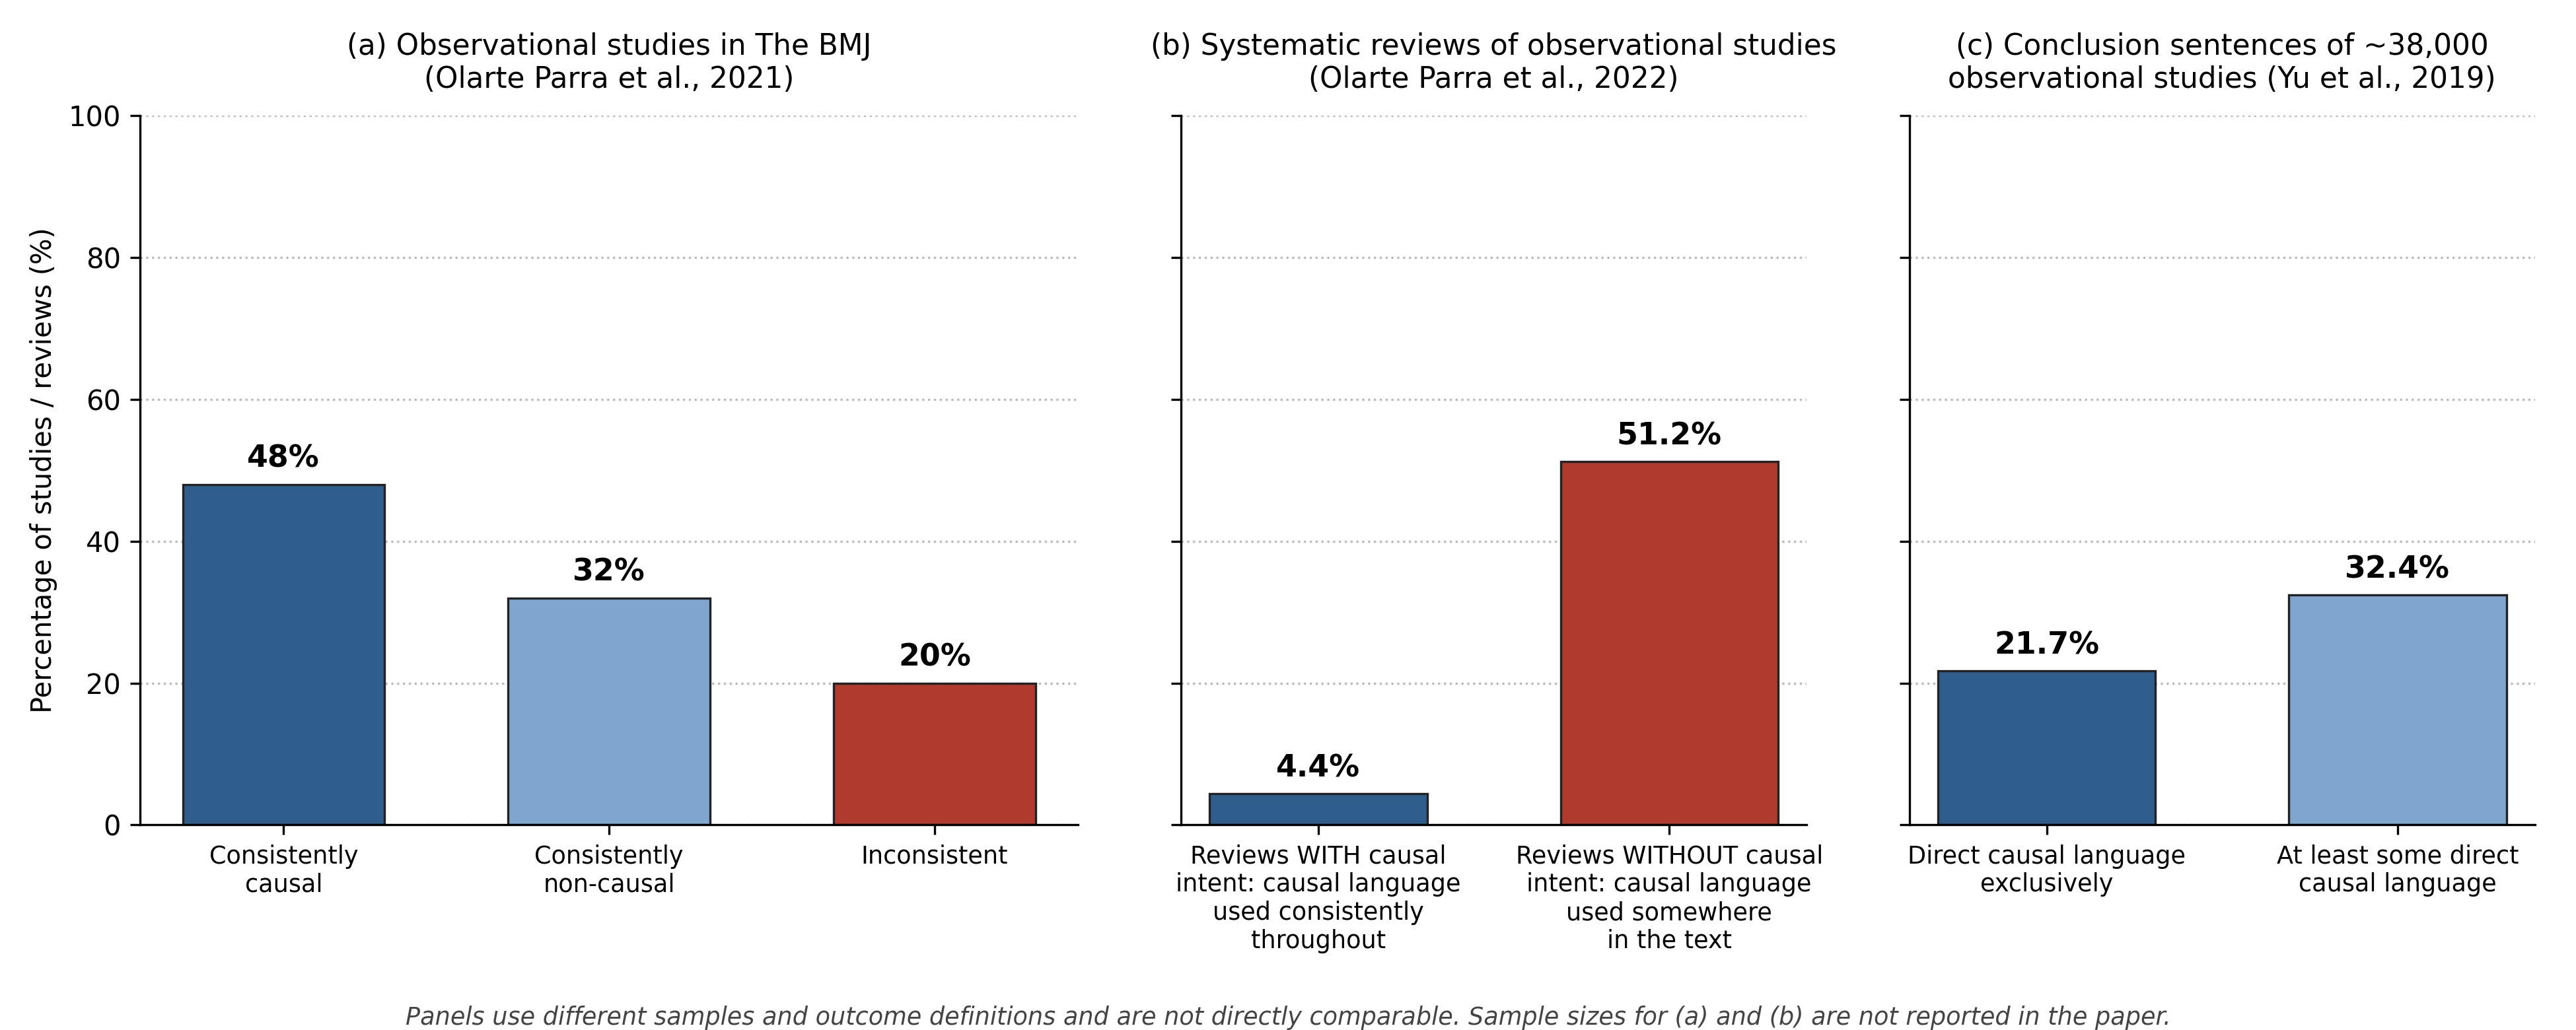
\includegraphics[width=\textwidth]{prism-uploads/Figure1_causal_language_prevalence_2.png}
  \caption{\textbf{Reported prevalence and inconsistency of causal language in prior studies.} (a) Share of observational studies in \textit{The BMJ} that were consistently causal, consistently non-causal, or inconsistent \cite{olarteparra2021}. (b) Systematic reviews of observational studies: percentage with causal intent that used causal language consistently, and percentage without causal intent that used causal language somewhere \cite{olarteparra2022}. (c) Direct causal language in the conclusions of approximately 38,000 observational studies \cite{yu2019}. Panels use different samples and definitions and are not directly comparable.}
  \label{fig:causal-language-prevalence}
\end{figure}

\subsection{LLMs and causal reasoning}

Evidence increasingly suggests that LLMs cannot be assumed to reliably distinguish semantic relatedness from causal explanation. Kim et al.~\cite{kim2023} evaluated ChatGPT on scientific and news claims categorized as causal, conditional causal, correlational, or unrelated. ChatGPT performed substantially worse than existing fine-tuned BERT models and had particular difficulty with conditional causal claims involving hedges.

More recent work provides a broader picture. Saklad et al.~\cite{saklad2026} evaluated LLM causal inference on real-world academic literature and reported substantial difficulty with causal relationships in complex texts; the best-performing model achieved an average F1 of 0.535 on their benchmark. Liu, Baraniuk, and Sonkar~\cite{liu2026clear}, using the CLEAR-3K benchmark, similarly found that LLMs frequently confuse semantic similarity with causal explanatory relationships.

Feng et al.~\cite{feng2025} further investigated LLM reliability for causal discovery and found limitations relevant to the use of LLMs as causal reasoning systems rather than merely language generators.

Together, these studies suggest that fluency should not be treated as evidence that an LLM has preserved causal semantics.

\section{Main Technical Discussion: Causal-Semantic Preservation as an Editing Constraint}
\label{sec:causal-semantic-preservation}

\subsection{Editing versus rewriting}

LLM-assisted editing should be distinguished from unrestricted generation. In a writing task, the user's implicit objective is often:
\[
  \begin{aligned}
    &\max_y && Q(y) \\
    &\text{subject to} && M(y,x)=1,
  \end{aligned}
\]
where $x$ is the source text, $y$ is the edited text, $Q$ measures qualities such as fluency and clarity, and $M$ represents semantic preservation.

For scientific editing, however, semantic preservation is multidimensional. At minimum, the system should preserve:

\begin{itemize}
  \item proposition content;
  \item direction of association or effect;
  \item population and scope;
  \item temporal relationship;
  \item study-design interpretation;
  \item uncertainty and hedging;
  \item modality;
  \item causal versus correlational status;
  \item strength of the claim;
  \item attribution of the claim;
  \item conditions under which the claim holds.
\end{itemize}

Thus:
\[
  M = (M_p,M_d,M_s,M_t,M_h,M_c,M_m,M_a).
\]
The causal component $M_c$ is particularly important because lexical changes can modify causal interpretation without changing the principal nouns or numerical values.

Figure~\ref{fig:causal-preservation-framework} presents the central causal-status preservation formulation.

\begin{figure}[htbp]
  \centering
  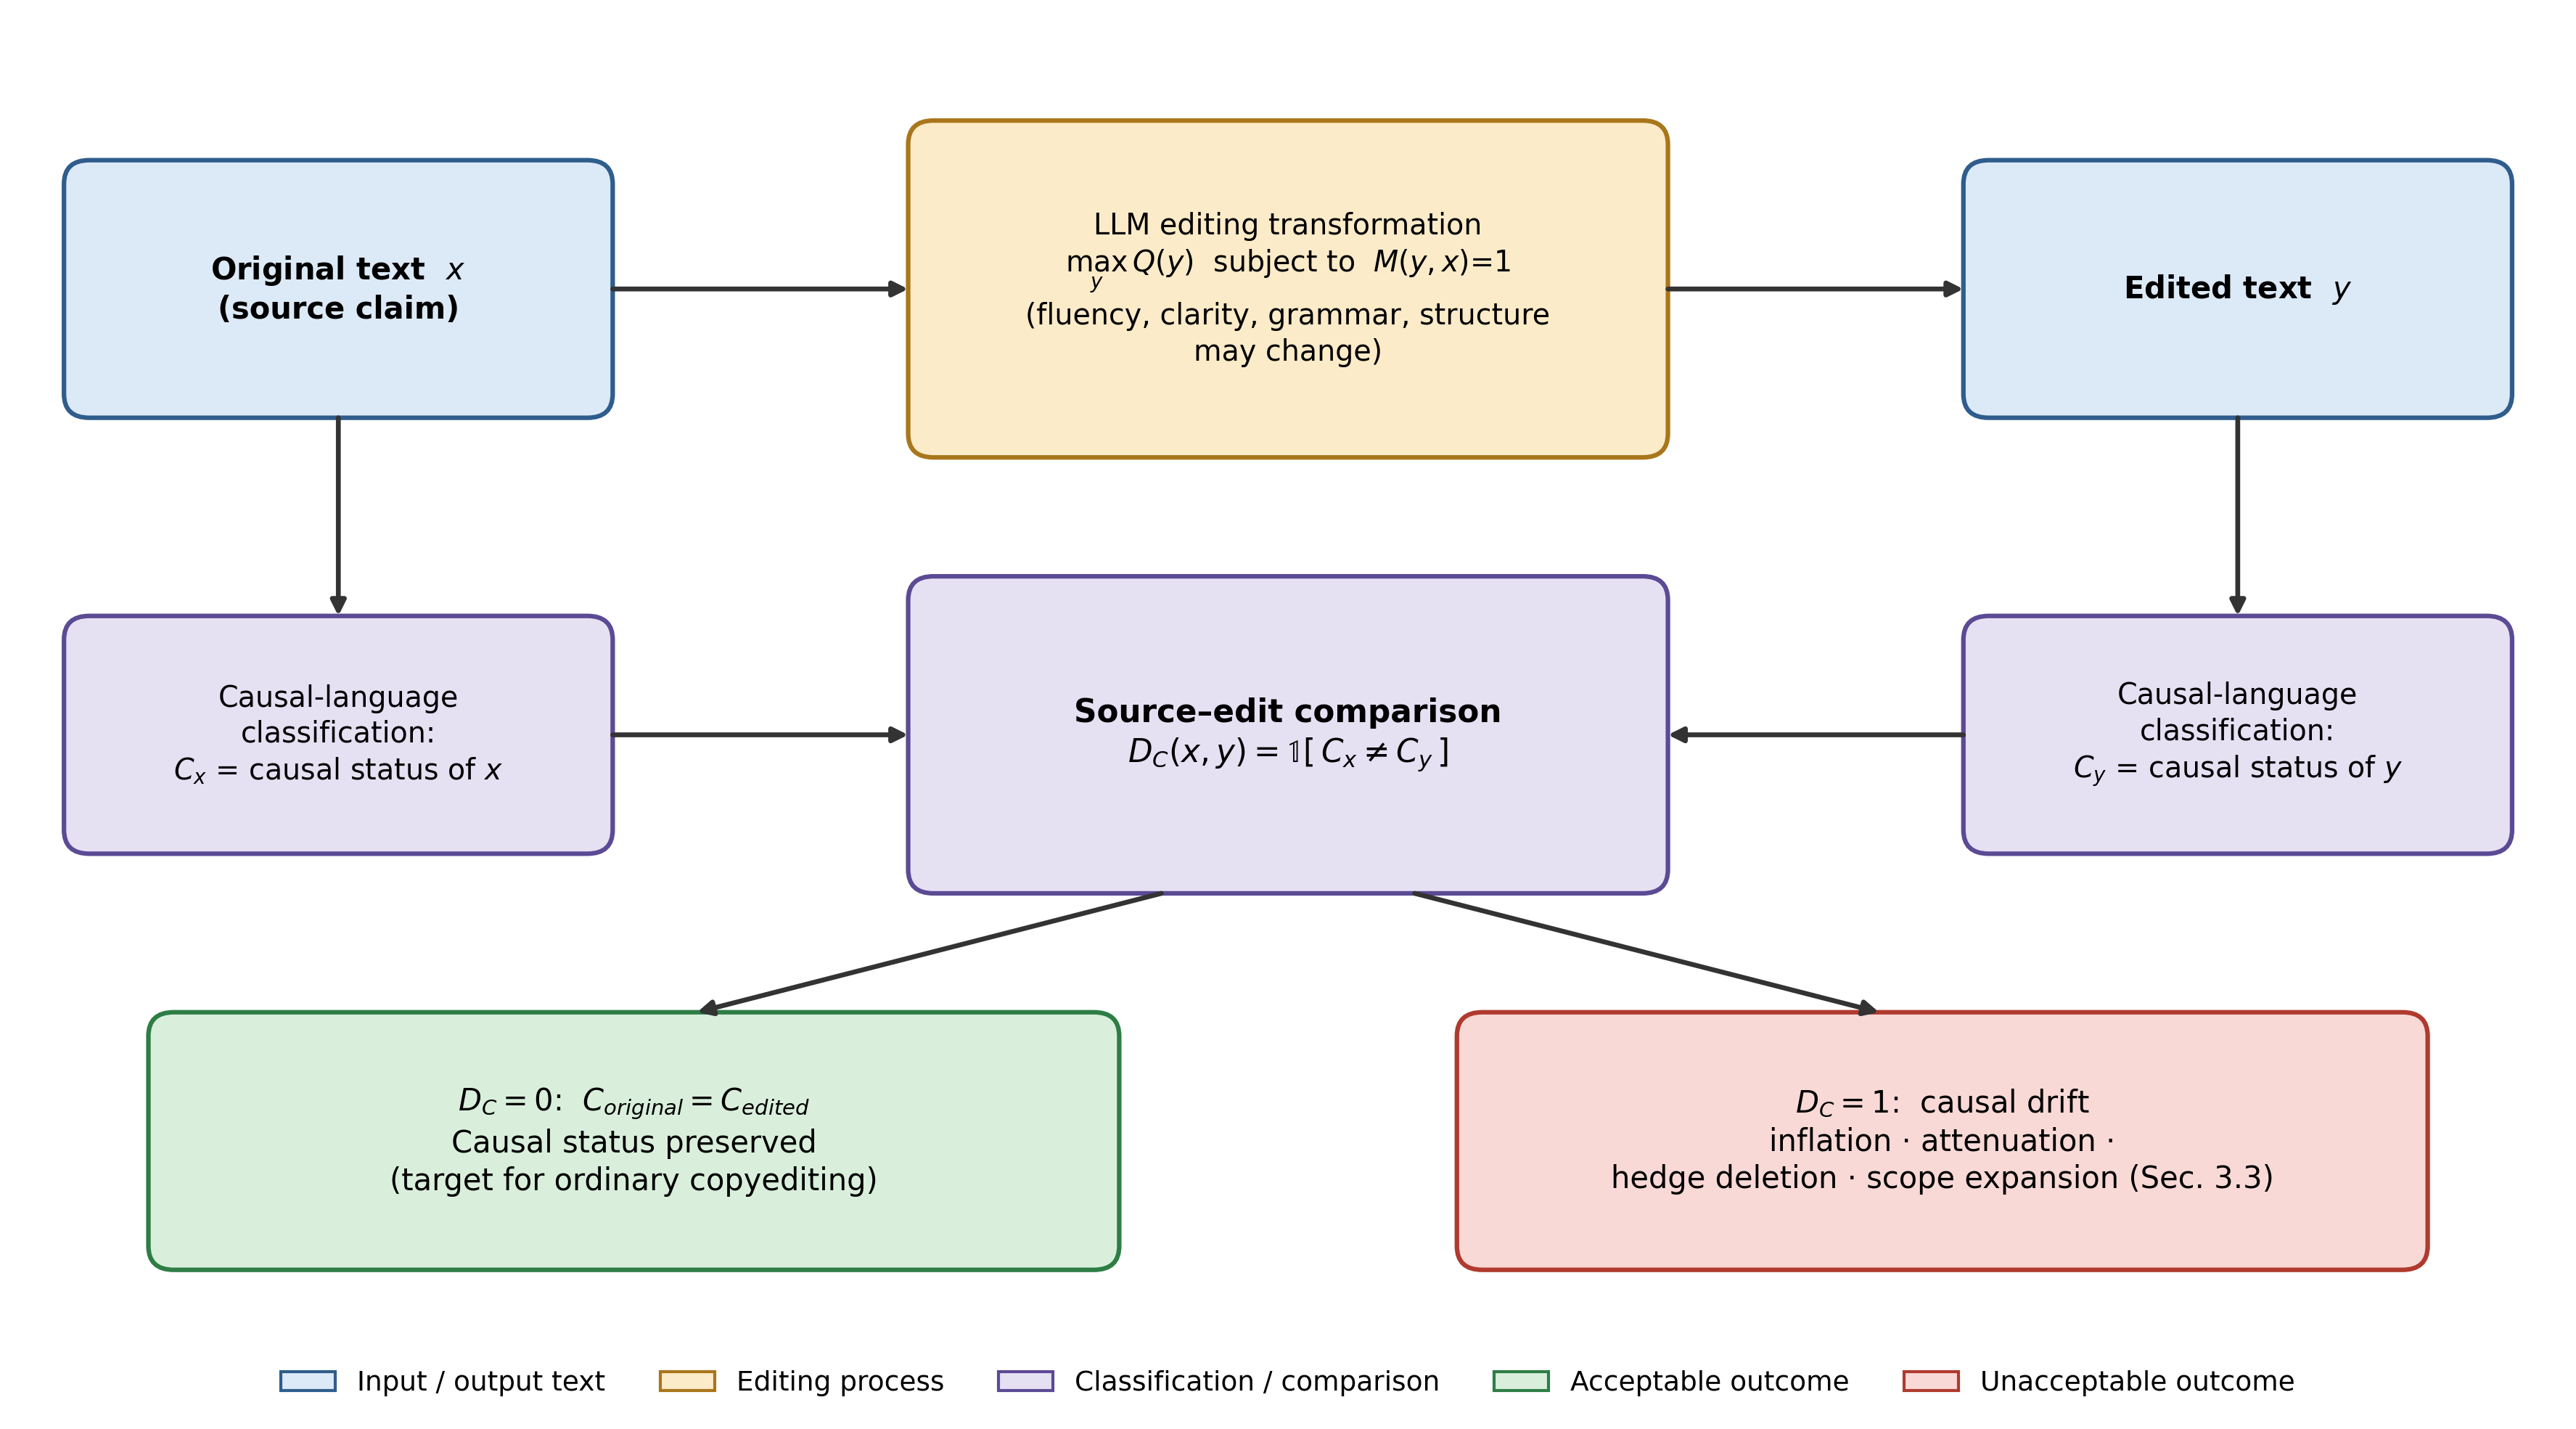
\includegraphics[width=0.95\textwidth]{prism-uploads/Figure2_causal_preservation_framework_2.png}
  \caption{\textbf{Conceptual framework for causal-status preservation in LLM-assisted editing.} The source text $x$ is edited to $y$ under a semantic-preservation constraint. Causal status is classified for both versions ($C_x$, $C_y$), and drift is $D_C = 1[C_x \neq C_y]$. Ordinary copyediting should yield $C_{\text{original}} = C_{\text{edited}}$.}
  \label{fig:causal-preservation-framework}
\end{figure}

\subsection{A causal-strength continuum}
\label{sec:causal-strength-continuum}

Causal language is not binary. Scientific prose can express several levels of epistemic and causal commitment:

Figure~\ref{fig:causal-strength-continuum} presents these levels and their examples.

\begin{figure}[htbp]
  \centering
  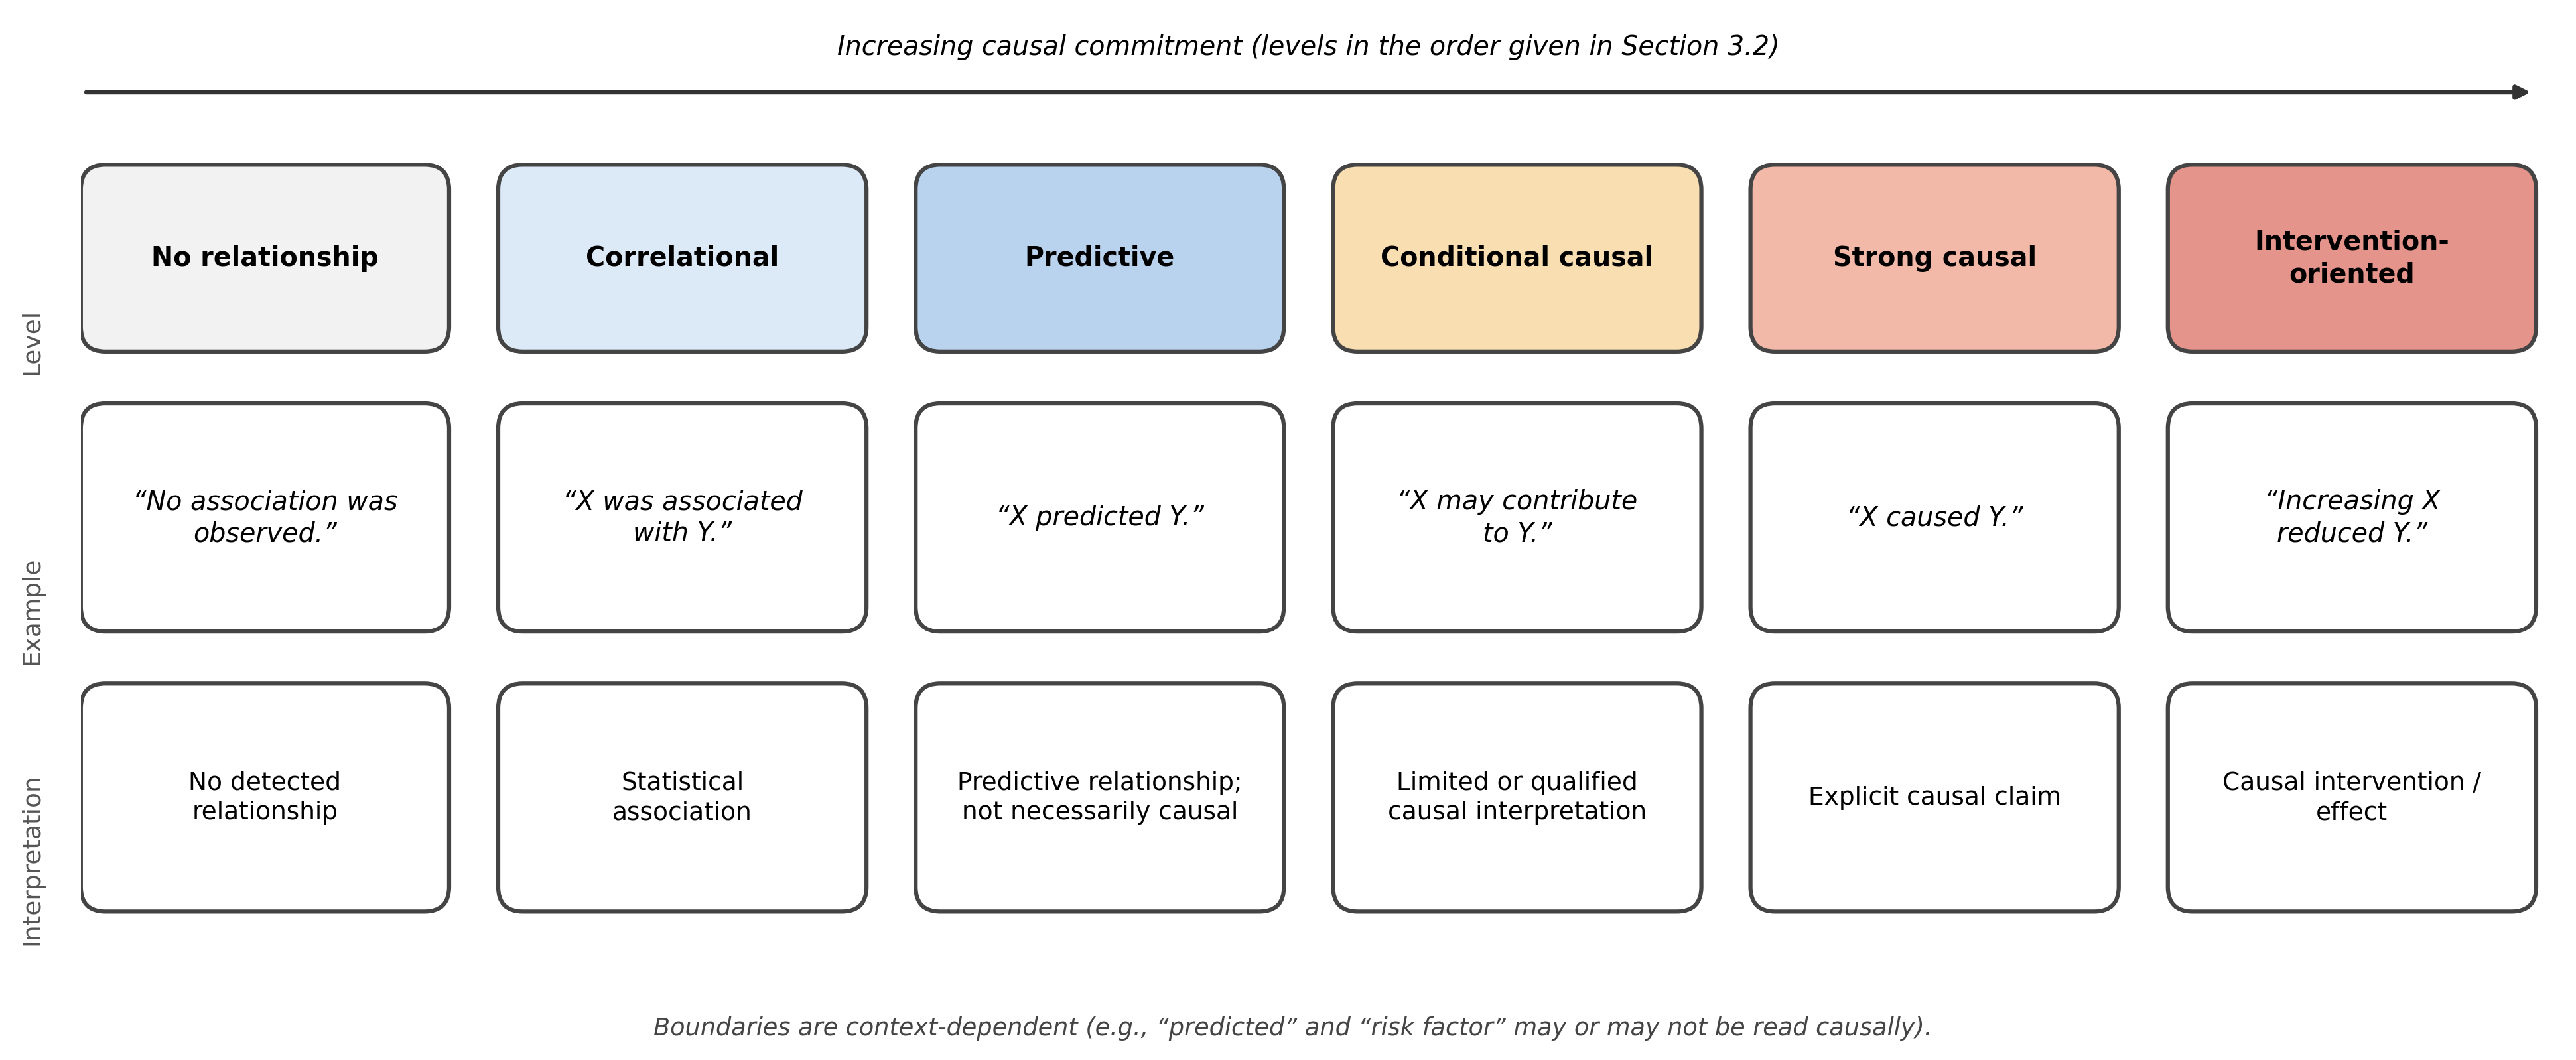
\includegraphics[width=\textwidth]{prism-uploads/Figure3_causal_strength_continuum_2.png}
  \caption{\textbf{Levels of causal commitment in scientific language.} Six levels with example sentences and typical interpretations, ordered as in Section~\ref{sec:causal-strength-continuum}. Boundaries are context-dependent; ``predicted'' and ``risk factor'' may or may not be read causally.}
  \label{fig:causal-strength-continuum}
\end{figure}

The boundaries are context-dependent. ``Predicted,'' for example, may be purely statistical or may be interpreted causally depending on the domain and surrounding text. Likewise, ``risk factor'' can carry causal implications even though it is frequently used ambiguously.

Reporting guidelines therefore emphasize that causal implications can be conveyed through terms such as ``effect,'' ``reduce,'' ``increase,'' and ``impact,'' rather than only through the word ``cause.''

A robust editor should consequently model causal strength as a structured property, rather than searching for individual causal keywords.

\subsection{Causal drift during paraphrasing}

Causal drift occurs when an editing operation changes the relationship between evidence and claim. Four common patterns can be distinguished.

Causal inflation occurs when an associational statement becomes causal:
\begin{quote}
Original: ``Exercise was associated with lower mortality.''

Edited: ``Exercise reduced mortality.''
\end{quote}

Causal attenuation occurs when a justified causal statement becomes merely associational:
\begin{quote}
Original: ``Randomization showed that the intervention reduced mortality.''

Edited: ``The intervention was associated with lower mortality.''
\end{quote}

Hedge deletion occurs when uncertainty disappears:
\begin{quote}
Original: ``The findings suggest that X may influence Y.''

Edited: ``X influences Y.''
\end{quote}

Scope expansion occurs when a qualified causal statement becomes general:
\begin{quote}
Original: ``Among adults with condition A, treatment X reduced symptom severity.''

Edited: ``Treatment X reduces symptoms.''
\end{quote}

These transformations are difficult to detect using conventional similarity metrics because the sentences may remain lexically and syntactically close.

\subsection{Why factuality is insufficient}

Traditional factuality evaluation asks whether an output is supported by a source. However, causal drift demonstrates that an output can contain all the same entities and approximate factual content while changing the type of inference.

For example, an original study may report an association between A and B. An edited sentence stating that A ``increased'' B may contain no false entity, date, or numerical value. Nevertheless, it asserts something stronger than the source establishes.

Consequently, LLM editing requires at least two separate dimensions:
\[
  \text{Fidelity}
  = \text{Propositional Fidelity}
  + \text{Epistemic/Causal Fidelity}.
\]
The latter cannot be reduced to conventional factual consistency.

\section{Current Approaches and Developments}
\label{sec:current-approaches}

\subsection{Causal-language classification}

The most direct approach is to classify source and edited sentences according to causal strength. The taxonomy developed by Yu et al.~\cite{yu2019}---nonrelationship, correlational, conditional causal, and direct causal---provides a useful foundation.

An editing system could classify both versions:
\[
  P(C \mid x), \qquad P(C \mid y)
\]
and calculate the causal-drift measure in Equation~\ref{eq:causal-drift}:
\begin{equation}
  \label{eq:causal-drift}
  D_C(x,y) = \mathbb{1}[C_x \neq C_y].
\end{equation}

A more sophisticated metric could penalize changes according to their direction and magnitude. Causal inflation should generally receive a different penalty from causal attenuation because the epistemic consequences differ.

\subsection{Prompt-based preservation}

A simple operational safeguard is to instruct the LLM explicitly:

\begin{quote}
``Improve grammar and clarity without changing whether any statement is causal, correlational, predictive, conditional, or uncertain. Preserve all hedges and causal qualifiers.''
\end{quote}

This strategy is attractive because it requires no model modification. However, Kim et al.~\cite{kim2023} demonstrate that prompt-based performance on causal-language tasks can vary with prompting conditions, and they caution against assuming that prompt engineering produces stable improvements across tasks and models.

Prompting should therefore be treated as a useful control layer rather than a guarantee.

\subsection{Claim-level intermediate representations}

A stronger architecture would first extract a structured representation of each scientific claim:
\[
  \langle \text{Subject}, \text{Predicate}, \text{Object}, \text{RelationType},
  \text{Qualifier}, \text{Population}, \text{Time}, \text{Evidence} \rangle.
\]

For example:
\[
  \langle \text{Exercise}, \text{associated-with}, \text{Mortality},
  \text{observational}, \text{Adults}, 5\text{ years}, \text{Cohort} \rangle.
\]

The LLM could then edit the prose while a separate verifier checks whether the structured claim remains unchanged.

This approach resembles the broader movement toward structured causal representations. Scientific claim-verification research has increasingly argued that causal structure should be explicitly represented rather than relying only on surface-level textual similarity (e.g., work on qualitative causal structures in scientific claims).

Figure~\ref{fig:claim-preserving-pipeline} shows how the proposed claim-extraction, verification, author-review, and provenance components fit together.

\begin{figure}[htbp]
  \centering
  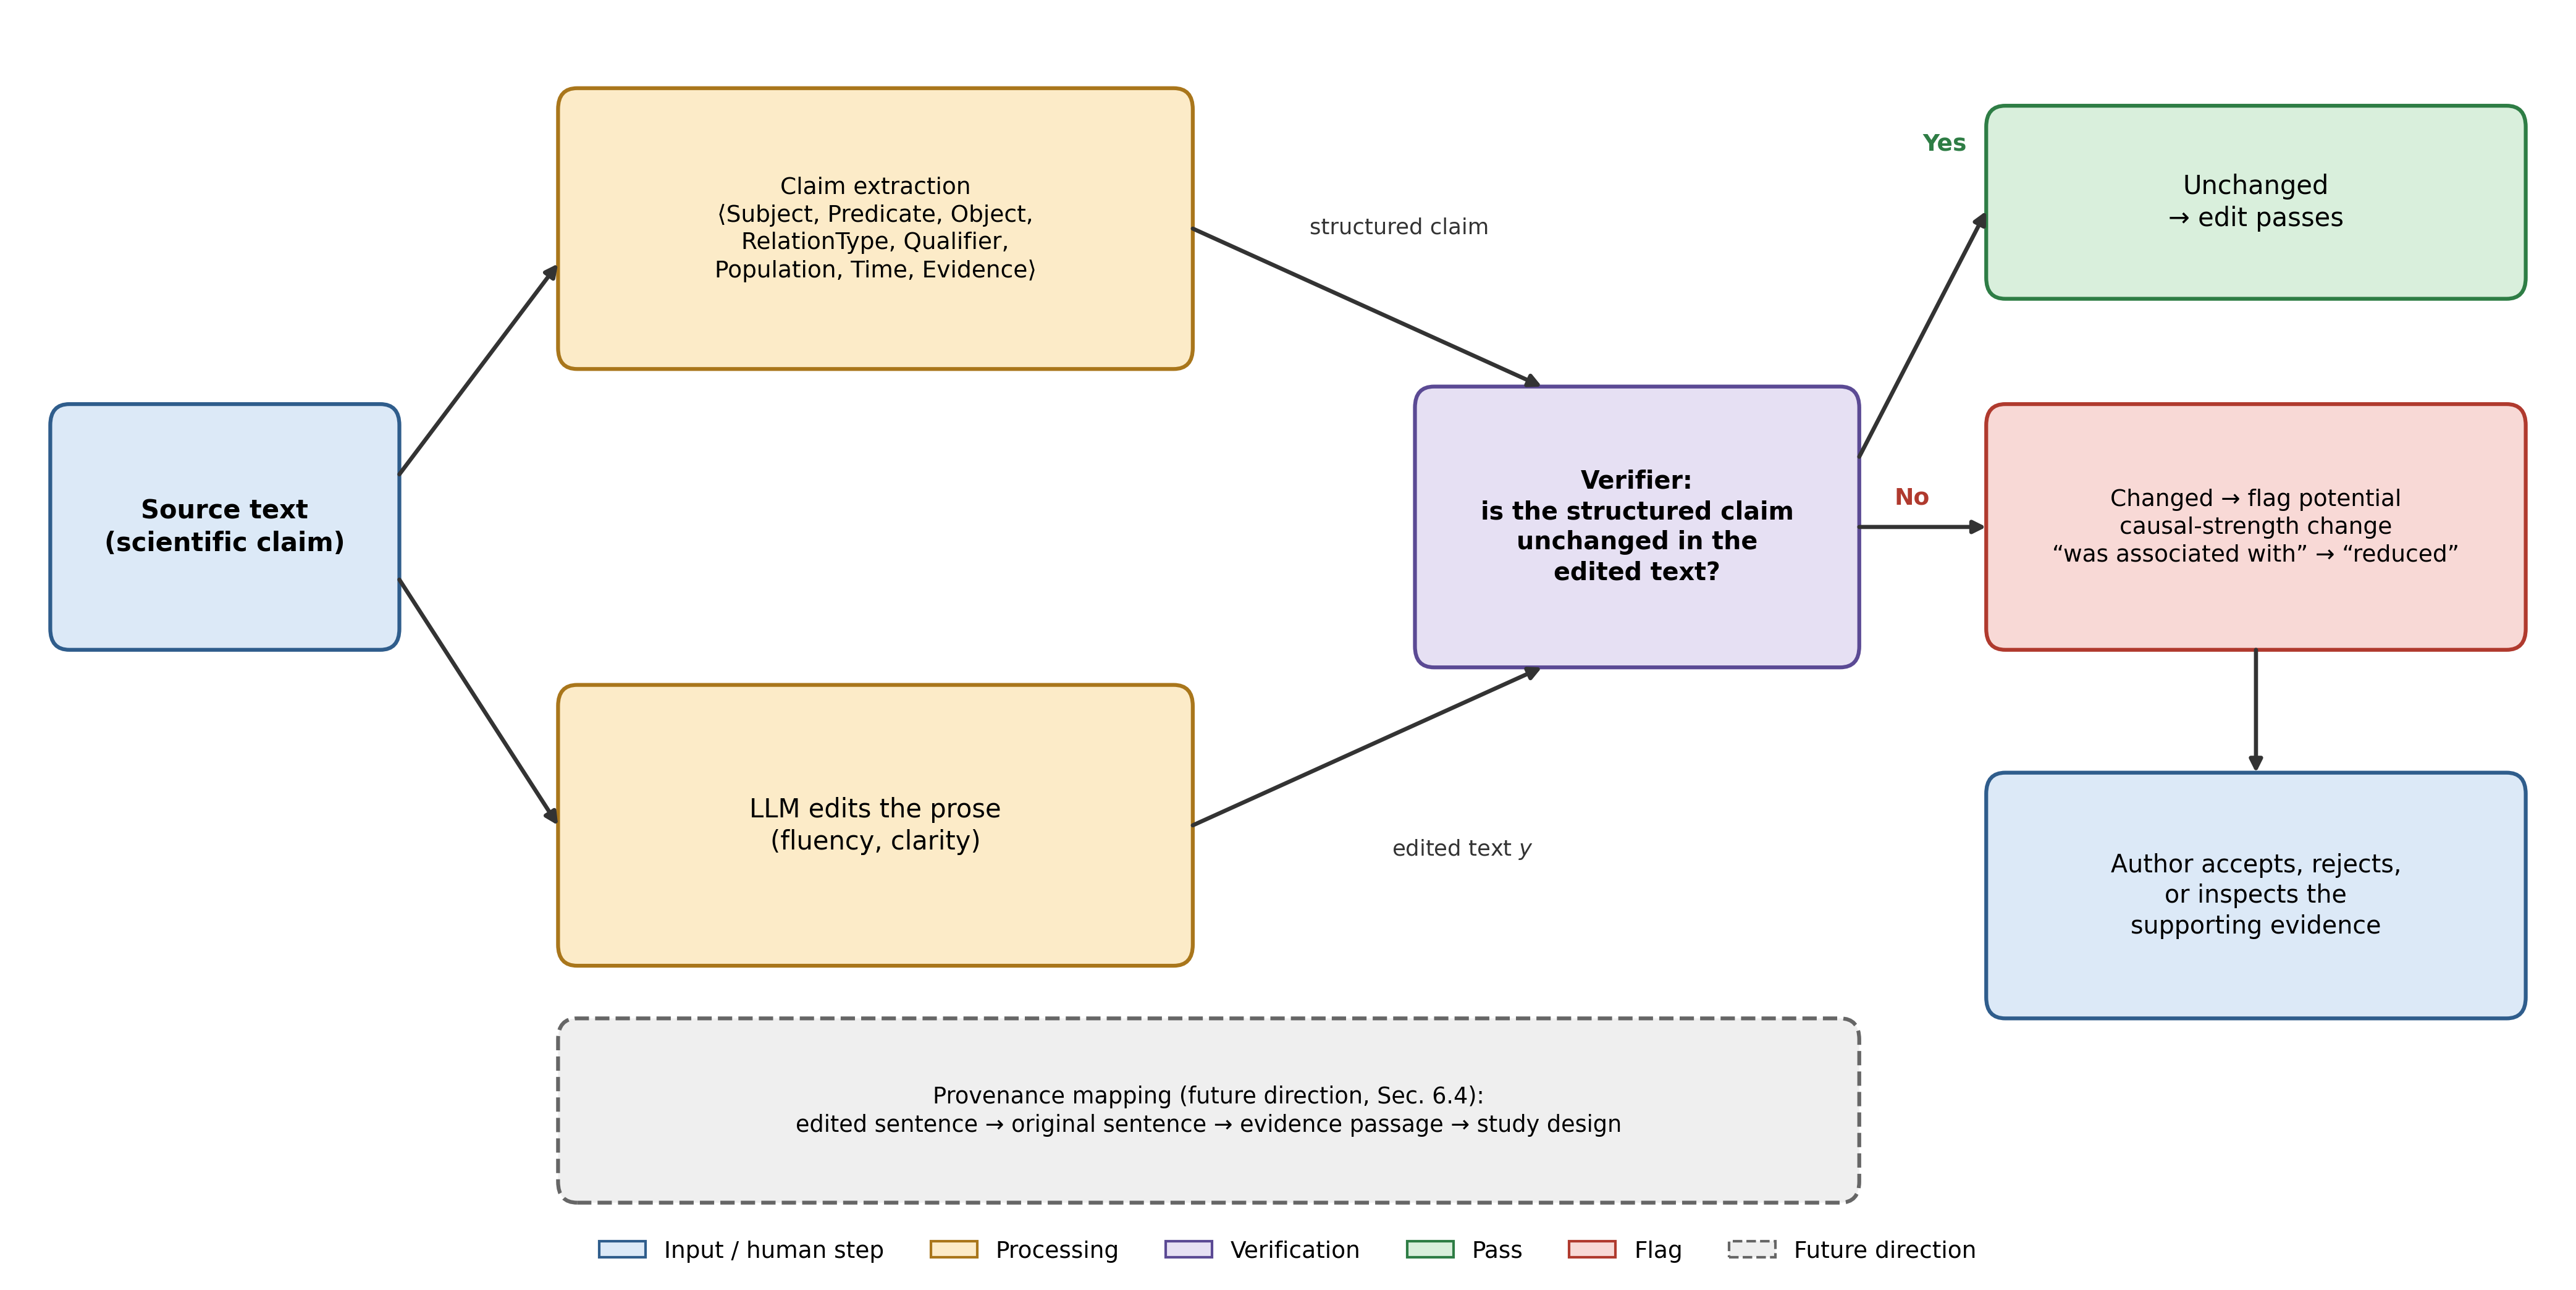
\includegraphics[width=\textwidth]{prism-uploads/Figure4_proposed_claim_preserving_pipeline.png}
  \caption{\textbf{Proposed claim-preserving editing pipeline.} A structured claim is extracted from the source. A verifier checks whether it is unchanged in the LLM-edited text. Changes are flagged for author review rather than silently applied. Provenance mapping (dashed) is a future direction. This architecture is conceptual and not evaluated in the paper.}
  \label{fig:claim-preserving-pipeline}
\end{figure}

\subsection{Human-in-the-loop verification}

Human review remains particularly important when editing changes verbs that carry causal implications. Rather than silently applying a transformation, an editing system could present:

\begin{quote}
Potential causal-strength change:

``was associated with'' $\rightarrow$ ``reduced''

This edit may strengthen the claim from correlational to causal.
\end{quote}

The user can then accept, reject, or inspect the supporting evidence.

Such interfaces would shift LLM editing from autonomous rewriting toward decision-support editing, preserving authorial responsibility.

\subsection{Claim verification and evidence alignment}

Causal preservation is also closely linked to claim verification. A sentence asserting that an intervention ``reduced'' an outcome should be evaluated against the study design, statistical analysis, and stated conclusions.

However, verification should not infer causality from study design alone. Randomized trials can have limitations, whereas observational analyses can sometimes support causal inference under explicit assumptions. Current reporting guidance increasingly emphasizes transparent causal assumptions rather than an absolute dichotomy between experimental and observational research.

\subsection{Knowledge editing and causal representations}

A parallel literature on editing the internal knowledge of LLMs is also relevant. Knowledge-editing research seeks to modify specific model behaviors or facts while minimizing unintended effects on unrelated knowledge \cite{yao2023}. Recent work has explicitly explored causal tracing and causally guided knowledge editing, illustrating growing interest in causal structure within model modification itself.

This literature is conceptually related but distinct from the present problem. Knowledge editing changes the model; causal-language preservation concerns changes in user-provided text. Nevertheless, techniques for tracing internal causal pathways may eventually contribute to more controllable editing systems.

\section{Research Challenges and Limitations}
\label{sec:research-challenges}

\subsection{Context dependence}

Causal meaning is highly context-dependent. ``Associated with,'' ``linked to,'' ``predicts,'' and ``drives'' do not have universally fixed causal interpretations. A sentence-level classifier can therefore fail when interpretation depends on previous paragraphs, methods, or study design.

\subsection{Domain variation}

Causal terminology differs across disciplines. Terms such as ``determinant,'' ``risk factor,'' ``effect modifier,'' ``driver,'' and ``mechanism'' have specialized meanings in epidemiology, economics, psychology, engineering, and social science.

A benchmark built entirely from biomedical literature may therefore overfit to one disciplinary discourse.

\subsection{Causal inference is not reducible to lexical choice}

Changing ``associated with'' to ``caused'' is clearly consequential, but the reverse problem is equally important: appropriate causal interpretation cannot be established by lexical analysis alone. Causal inference depends on assumptions, identification strategies, design, measurement, confounding, selection, and counterfactual interpretation \cite{pearl2009}.

Thus, causal-language preservation should not become an automated system for deciding whether authors deserve to make causal claims. Its primary task should be to preserve the author's explicitly supported claim unless substantive revision is requested.

\subsection{Ambiguous hedging}

Scientific writing frequently uses modal expressions such as ``may,'' ``might,'' ``could,'' ``suggests,'' ``is consistent with,'' and ``is likely.'' These expressions encode uncertainty, but their exact epistemic force is context-dependent.

Kim et al.~\cite{kim2023} found that ChatGPT had particular difficulty with conditional causal claims involving hedges. This suggests that preservation benchmarks must explicitly include hedged claims rather than focusing only on clear ``cause'' versus ``association'' contrasts.

\subsection{Evaluation difficulties}

BLEU, ROUGE, BERTScore, semantic similarity, and general factuality metrics are not sufficient for this task. An edited sentence can score highly on semantic similarity while changing causal status.

A suitable evaluation suite should therefore include:

\begin{itemize}
  \item causal-status accuracy;
  \item causal-strength distance;
  \item hedge preservation;
  \item directionality preservation;
  \item population/scope preservation;
  \item evidence-to-claim alignment;
  \item human judgments by domain experts.
\end{itemize}

\subsection{Model and version dependence}

LLM behavior changes rapidly across models and versions. A benchmark demonstrating preservation in one model does not establish preservation generally. This is particularly relevant because recent studies report substantial differences in causal reasoning across models and model sizes \cite{liu2026clear,saklad2026}.

\section{Research Gaps and Future Directions}
\label{sec:research-gaps}

\subsection{A dedicated causal-preservation benchmark}

There is a clear need for a benchmark specifically designed around editing, rather than causal reasoning or causal extraction alone.

Each benchmark item could contain:

\begin{enumerate}
  \item an original scientific sentence;
  \item study-design information;
  \item the author's intended causal status;
  \item an LLM-edited version;
  \item expert annotations of whether causal force was preserved;
  \item acceptable and unacceptable alternative edits.
\end{enumerate}

The benchmark should include causal inflation, attenuation, hedge deletion, scope expansion, and direction reversal.

\subsection{Counterfactual semantic evaluation}

One promising evaluation method is to ask whether the edited sentence implies the same answer to controlled counterfactual questions.

For example:

\begin{quote}
Original:

``X was associated with higher Y.''

Counterfactual test:

``Does the sentence imply that intervening to increase X would increase Y?''

Expected answer: No---not necessarily.
\end{quote}

An edited version that produces Yes would exhibit causal inflation.

This provides a more principled test than lexical matching.

Figure~\ref{fig:counterfactual-semantic-test} illustrates the counterfactual semantic test.

\begin{figure}[htbp]
  \centering
  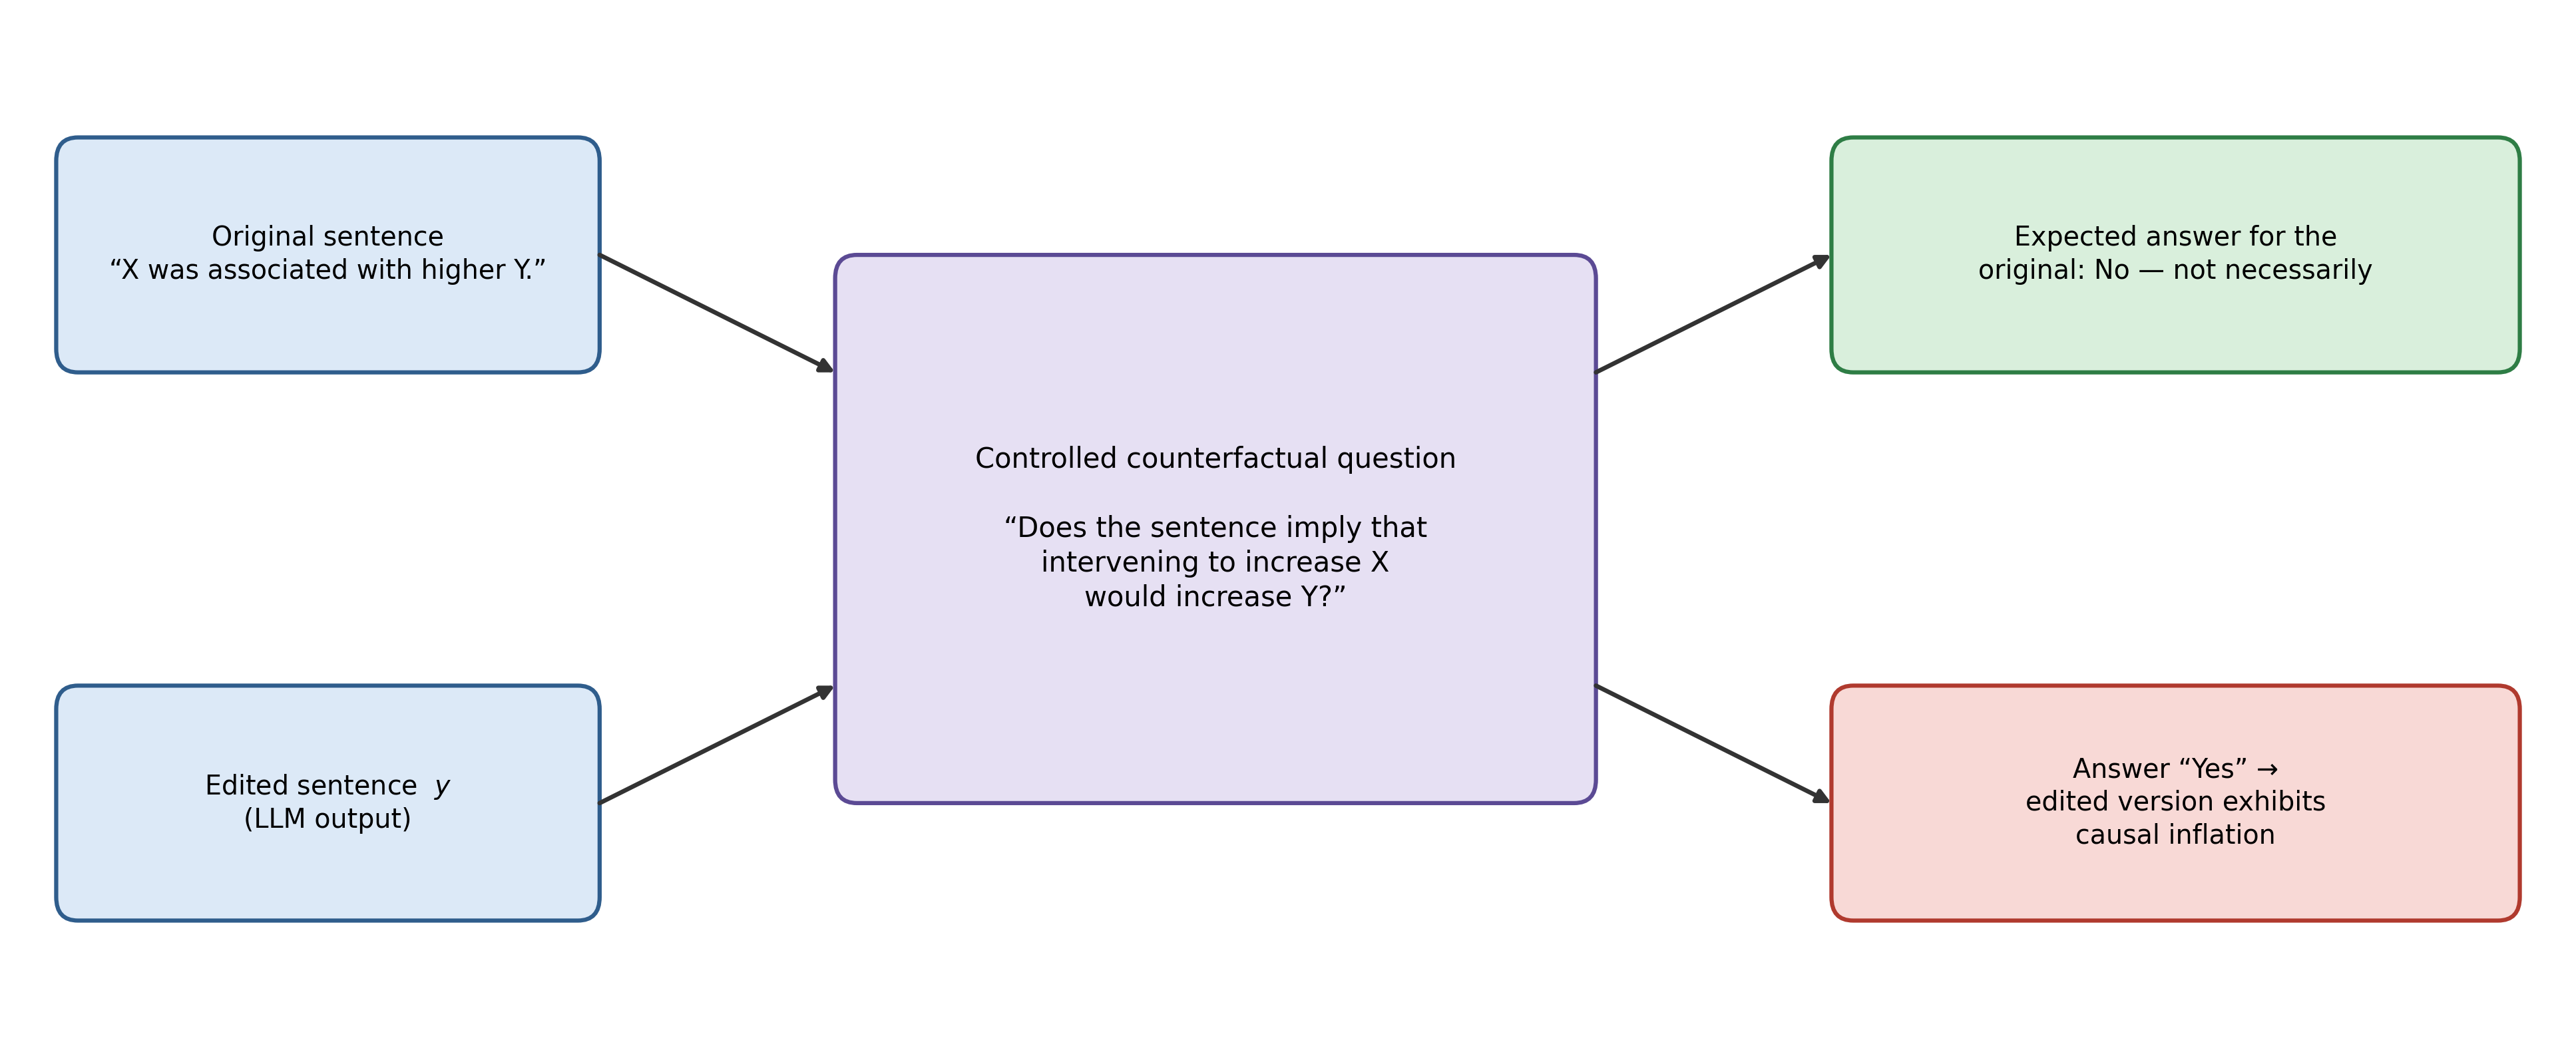
\includegraphics[width=\textwidth]{prism-uploads/Figure5_counterfactual_semantic_test_2.png}
  \caption{\textbf{Counterfactual semantic test for causal inflation.} The original and edited sentences are probed with the same counterfactual question. A ``Yes'' for an edit of ``X was associated with higher Y'' indicates causal inflation.}
  \label{fig:counterfactual-semantic-test}
\end{figure}

\subsection{Causal graphs as editing constraints}

Where sufficient methodological information exists, an editor could represent the study as a directed acyclic graph (DAG). The language generator could then be constrained by the identified causal structure.

For instance, if the text describes an observational association between $X$ and $Y$ confounded by $Z$, the editing system could be prohibited from generating language implying an unqualified $X \rightarrow Y$ effect.

This connects scientific editing with established causal-graph methodology and may substantially improve semantic control.

\subsection{Provenance-aware editing}

Future systems should retain a mapping between each edited claim and its source evidence:
\[
  \text{Edited sentence}
  \rightarrow \text{Original sentence}
  \rightarrow \text{Evidence passage}
  \rightarrow \text{Study design}.
\]

Such provenance would enable an editor to explain why a proposed causal verb is potentially problematic.

\subsection{Interactive epistemic controls}

Rather than providing a single rewritten sentence, an LLM could offer explicitly categorized alternatives:

\begin{itemize}
  \item Meaning-preserving: ``was associated with''
  \item More cautious: ``was weakly associated with''
  \item Potentially causal: ``may have contributed to''
  \item Strong causal: ``reduced''
\end{itemize}

The system should identify which alternatives change the epistemic status of the claim.

\subsection{Multilingual causal-language preservation}

Most existing resources are concentrated in English. Yet causal semantics are expressed differently across languages, and translation itself can alter evidential and modal distinctions.

Future research should construct multilingual causal-editing datasets and examine whether LLMs preserve causal status across translation and subsequent editing.

\subsection{Integration into scholarly writing infrastructure}

Because LLM-assisted writing is increasingly common in academic publishing, causal-semantic verification could be integrated into word processors, manuscript-management systems, and journal submission platforms. Recent guidance on ethical LLM use emphasizes transparency and human responsibility in academic writing rather than treating LLMs as autonomous authors \cite{porsdammann2024}.

The ideal system would therefore function as a semantic integrity layer between author and LLM.

Table~\ref{tab:empirical-evidence} summarizes the empirical findings on causal-language use and LLM-associated writing reported in the studies discussed in Sections~\ref{sec:introduction}, \ref{sec:causal-language-inconsistency}, and~\ref{sec:causal-language-detection}.

\begin{table}[htbp]
  \centering
  \caption{Empirical evidence on causal-language use and LLM-associated writing in the literature.}
  \label{tab:empirical-evidence}
  \begin{minipage}{\textwidth}
    \small
    Summary of published findings on causal-language consistency in scientific reports and on the prevalence of LLM-associated vocabulary in biomedical abstracts. Samples and outcome definitions differ across studies.
  \end{minipage}
  \vspace{0.5em}

  \footnotesize
  \renewcommand{\arraystretch}{1.2}
  \setlength{\tabcolsep}{4pt}
  \begin{tabularx}{\textwidth}{@{}>{\raggedright\arraybackslash}p{0.18\textwidth}
                                  >{\raggedright\arraybackslash}p{0.24\textwidth}
                                  >{\raggedright\arraybackslash}p{0.23\textwidth}
                                  >{\raggedright\arraybackslash}X@{}}
    \toprule
    \textbf{Study} & \textbf{Data} & \textbf{Outcome} & \textbf{Reported result} \\
    \midrule
    Olarte Parra et al.~\cite{olarteparra2021}
      & Observational studies in \textit{The BMJ} (sample size not reported in the paper)
      & Consistency of causal language across objectives, methods, results, conclusions
      & 48\% consistently causal; 32\% consistently non-causal; 20\% inconsistent \\
    \addlinespace
    Olarte Parra et al.~\cite{olarteparra2022}
      & Systematic reviews of observational studies (sample size not reported)
      & Agreement between causal intent and causal language
      & Reviews with causal intent: 4.4\% used causal language consistently throughout. Reviews without causal intent: 51.2\% used causal language somewhere \\
    \addlinespace
    Yu, Li \& Wang~\cite{yu2019}, applied model
      & $\sim$38,000 observational studies
      & Causal language in conclusions
      & 21.7\% used direct causal language exclusively; 32.4\% used at least some \\
    \addlinespace
    Kobak et al.~\cite{kobak2025}
      & $>$15 million PubMed abstracts
      & Textual signals associated with LLM processing
      & At least 13.5\% of 2024 abstracts (a lower bound, not identification of individual LLM use) \\
    \bottomrule
  \end{tabularx}
\end{table}

\section{Conclusion}
\label{sec:conclusion}

Preserving causal versus correlational language during LLM-assisted editing is a specialized form of semantic fidelity with direct implications for scientific communication. The distinction between association and causation is foundational to causal inference, and scientific reporting literature demonstrates that humans already struggle to maintain consistent causal framing. LLMs add a new source of risk because their principal strength---fluent, context-sensitive paraphrasing---can inadvertently modify epistemic force.

Existing causal-language classifiers demonstrate that causal status can be computationally identified, while recent studies show that LLMs themselves remain imperfect at distinguishing semantic relatedness from causal explanation. Recent evidence that LLMs can amplify causal overstatement in scientific summaries makes the problem particularly important for automated editing and summarization systems.

The appropriate objective is not to prohibit causal language or to force all observational findings into non-causal formulations. Rather, LLM-assisted editing should preserve the relationship between evidence, inference, and linguistic strength. A scientifically responsible editing system should improve clarity while maintaining causal status, uncertainty, scope, directionality, and evidential qualification.

Future systems should therefore move beyond generic notions of factuality and semantic similarity toward explicit causal-semantic constraints, claim-level provenance, structured causal representations, counterfactual evaluation, domain-aware benchmarks, and human-in-the-loop review. The central design principle is straightforward: an LLM may change how a scientific claim is expressed without silently changing what the evidence permits the claim to mean.

\bibliographystyle{plain}
\bibliography{references}

\end{document}
